%%% Sekce - Interaktivní mapa
%%%%% Wording: ✅
%%%%% Styling: ✅
%%%%% References: ✅
%%%%% Grammar: ✅
%%% --------------------------------------------------------------
\section{Interaktivní mapa}
\label{sec:identifikace-interaktivni-mapa}
Vizualizace a celkové zobrazení interaktivní mapy sedaček místa konání akce je jednou z nejdůležitějších částí celého systému.
Tato sekce se zabývá nejhlavnějšími aspekty vizualizace mapy sedaček, jako je celkové rozvržení a struktura, barevné kódování prvků na mapě, ovládání mapy, zobrazení dostupných informací o zvoleném místě a také důležitost dostupnosti dat v~reálném čase.
V každé sekci budou tyto aspekty podrobněji rozebrány, ukázány příklady z reálného světa a vysvětlena jejich důležitost.

%%% Podsekce - Rozložení a struktura
%%%%% Wording: ✅
%%%%% Styling: ✅
%%%%% References: ✅
%%%%% Grammar: ✅
%%% --------------------------------------------------------------
\begin{subsection}{Rozložení a struktura}
    \label{subsec:identifikace-interaktivni-mapa-rozlozeni-a-struktura}
    Pro docílení přehledného a uživatelsky přívětivého zobrazení plánku sedaček je třeba zajistit správnou vizuální strukturu a ideální rozložení prvků na obrazovce.
    Dobře uspořádané uživatelské rozhraní pomáhá zákazníkům lépe se v mapě orientovat a vybrat tak preferovaná místa rychleji a snadněji.

    Obrázek~\ref{fig:venue-map-visualization-layout-and-structure} zobrazuje příklad zasedacího pořádku portálu Ticketportal.cz v Divadle U Hasičů v Praze na Vinohradech.
    V tomto zobrazení nalezneme indikaci hlediště, dostupných i nedostupných míst k sezení a číslování řad sedaček.
    Toto zobrazení, ačkoliv poskytuje všechny důležité informace, není tolik uživatelsky přívětivé a atraktivní.
    Například výběr správně kontrastního barevného zobrazení sedaček by celkovému zobrazení velmi prospělo.
    Problematiku barevného kódování dále rozebírá následující sekce~\ref{subsec:identifikace-interaktivni-mapa-barevne-kody}.

    \begin{figure}[H]
        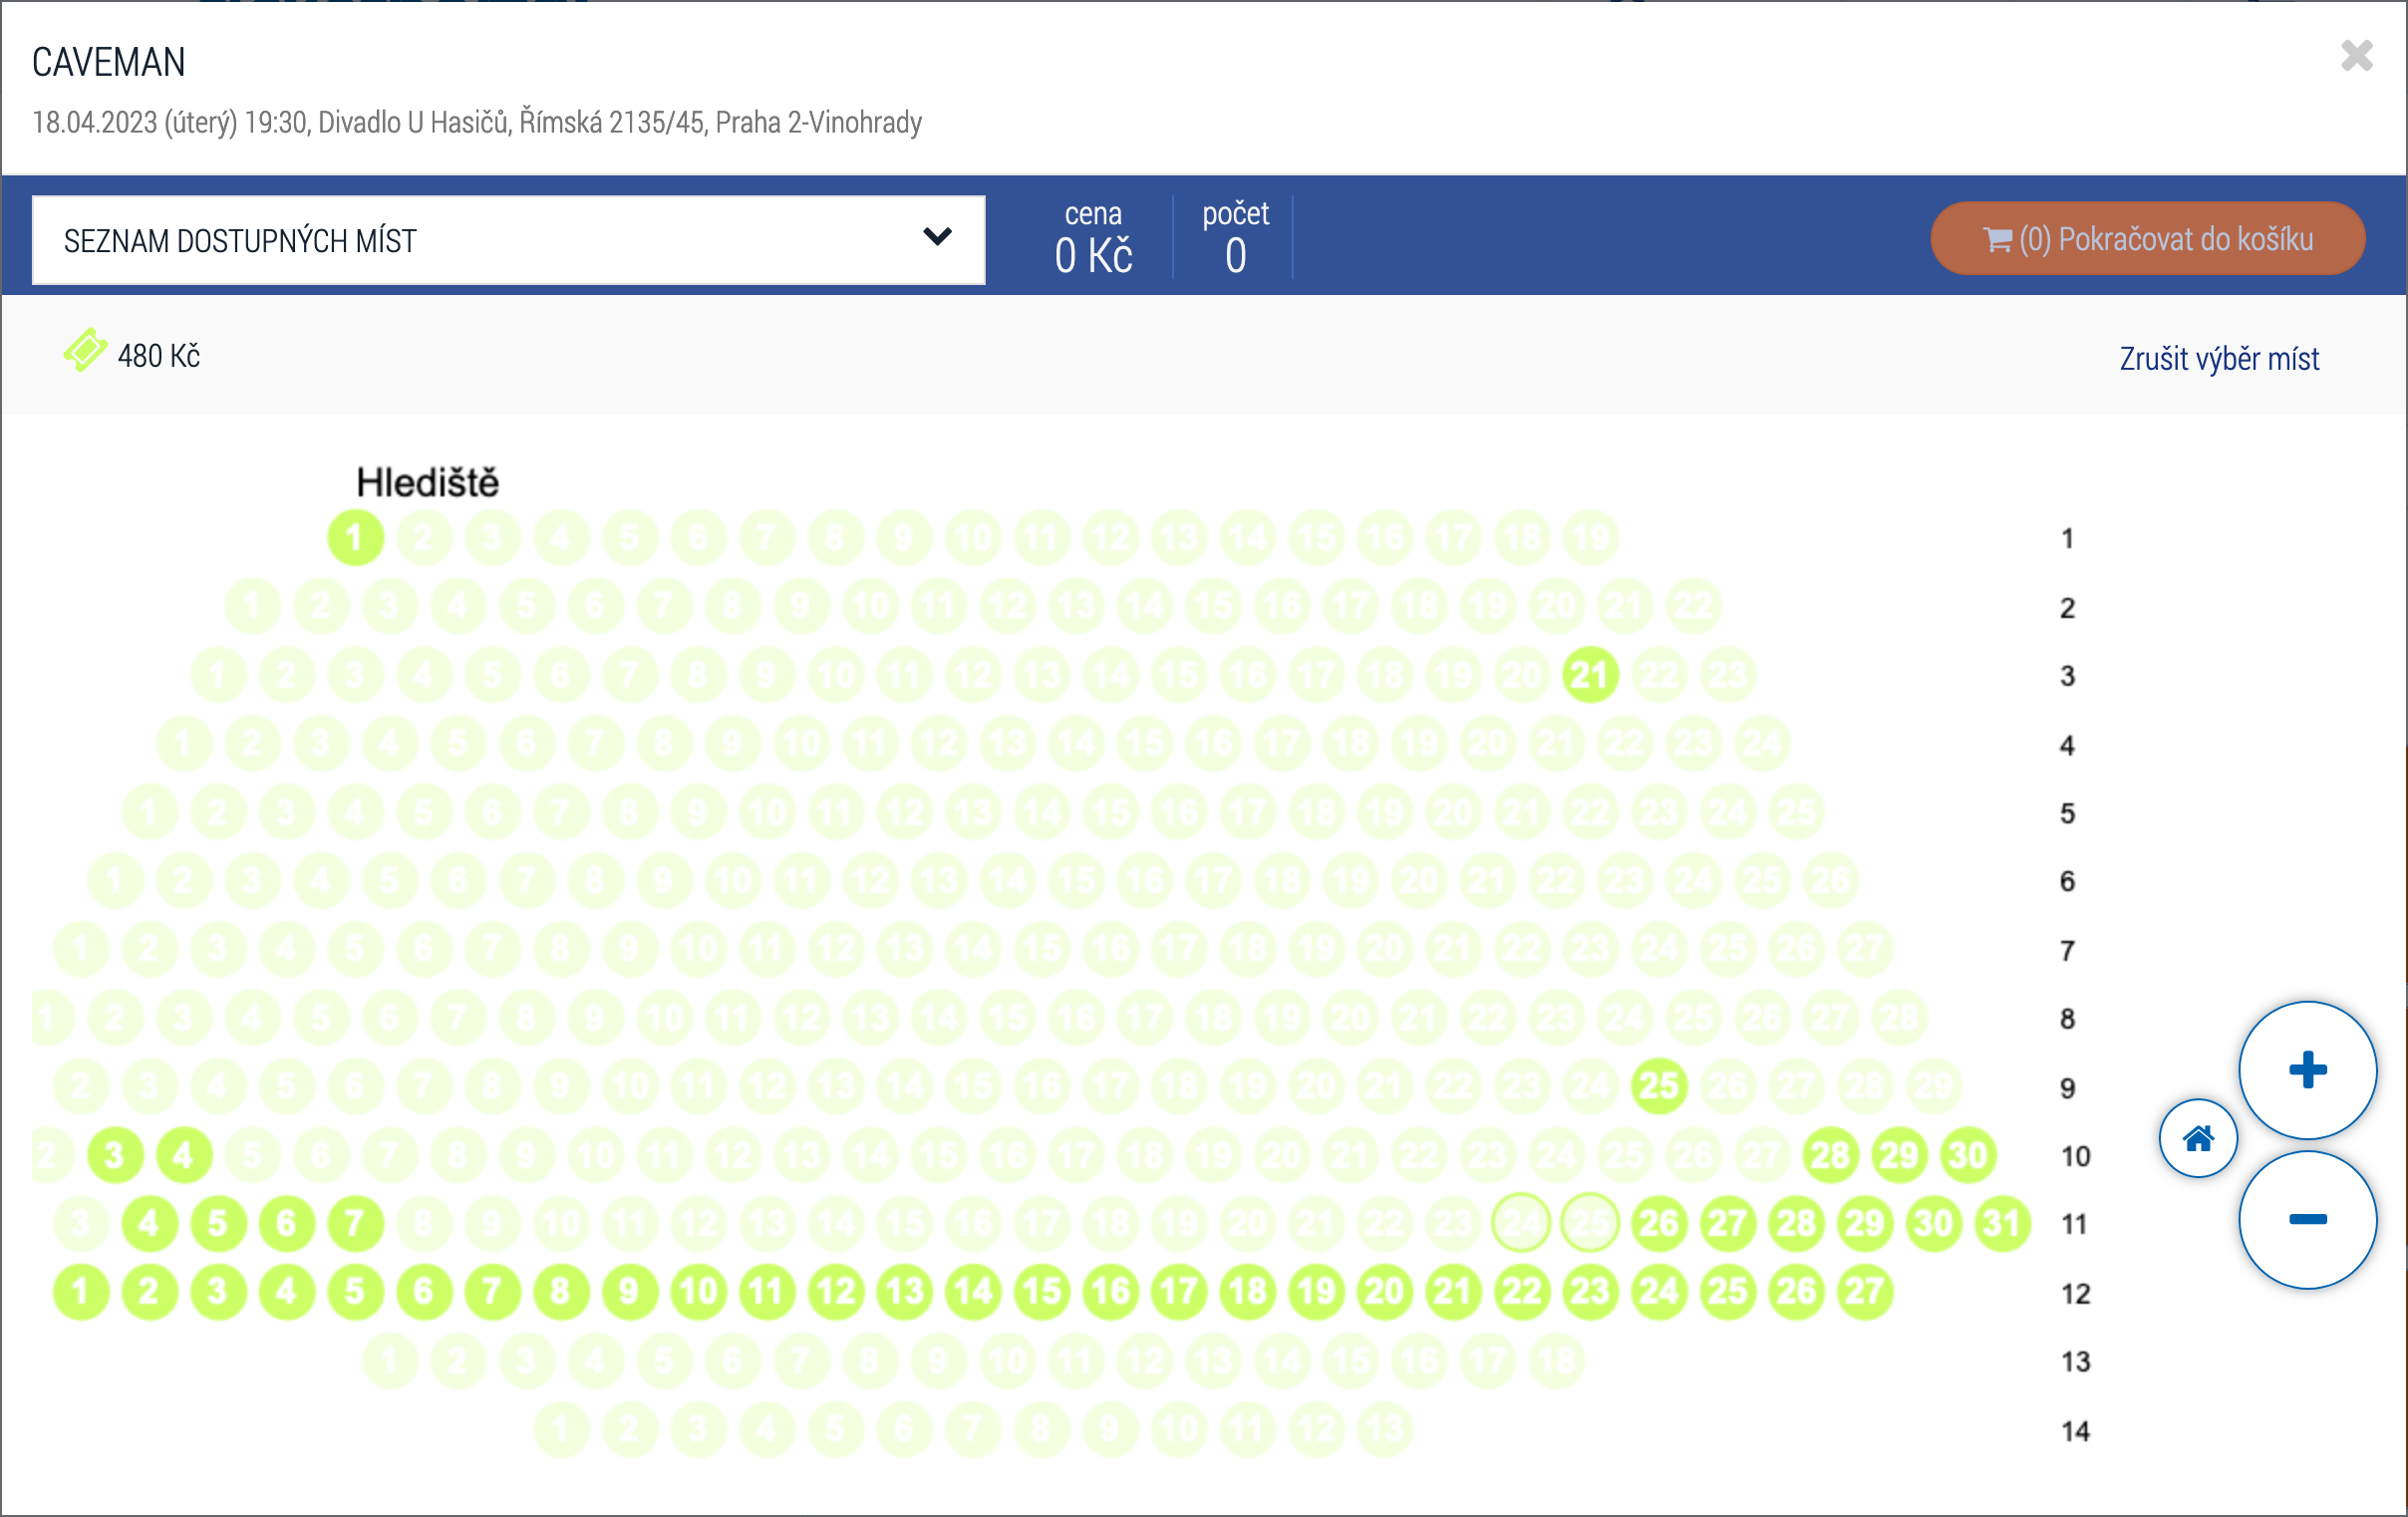
\includegraphics[width=\linewidth]{\FIGDIR/ticketportal-divadlo-u-hasicu}
        \centering
        \caption{Plánek sedaček v síti Ticketportal.cz\cite{t__www_ticketportal_cz}}
        \label{fig:venue-map-visualization-layout-and-structure}
    \end{figure}

    Rozložení a struktura prvků na mapě by měly upřednostňovat uživatelskou přívětivost a snadnou navigaci, aby zákazníci mohli rychle najít a vybrat požadovaná místa.
    Aby bylo tohoto dosaženo, měla by vizualizace mapy zahrnovat zřetelné sekce, jasné popisky a intuitivní uspořádání míst k sezení či případně i místa vymezená pro stání.

    Nejdůležitější prvky, které by mapa měla obsahovat jsou:
    \begin{enumerate}
        \item \textbf{Místa k sezení} – zvýrazněná místa k sezení, která jsou k dispozici pro výběr.
        \item \textbf{Místa pro stání} – místa, která jsou určena pro stání, mají větší kapacitu než místa k sezení a jsou také k dispozici pro výběr.
        \item \textbf{Sektory} – rozdělení větších plánku se sedačkami do jednotlivých sektorů seskupujících místa k sezení či stání.
        \item \textbf{Hlediště} – místo, kam budou hledět návštěvníci, důležité pro výběr místa s dobrým výhledem.
        \item \textbf{Popisky} – popisky pro zvýraznění významných míst, jako třeba řady nebo názvy sekcí.
        \item \textbf{Značky pro zvýraznění dalších objektů} – méně důležité, přesto informativní prvky na mapě jako třeba WC, bar, kavárna nebo zábradlí či sloupy.
    \end{enumerate}

    Tyto prvky by měli být jasně vizuálně definované a na mapě přehledně rozložené.
    Záleží převážně o správnou definici a nakreslení prvků na mapě, což je úzce spojeno s administrací mapy a jejího nastavení.
    Tu totiž musí někdo prvně vydefinovat a uložit do nějakého datového formátu.
    Data si v tomto formátu poté vyžádá aplikace a na jejich základě mapu vykreslí uživateli v prohlížeči.
    Touto problematikou se následně více zabývá sekce~\ref{sec:implementace-seating} v implementační části práce.
\end{subsection}

%%% Podsekce - Barevné kódování
%%%%% Wording: ✅
%%%%% Styling: ✅
%%%%% References: ✅
%%%%% Grammar: ✅
%%% --------------------------------------------------------------
\begin{subsection}{Barevné kódování}
    \label{subsec:identifikace-interaktivni-mapa-barevne-kody}
    Barevné kódování je dalším zásadním aspektem vizuálního zobrazení mapy místa konání, jelikož pomáhá uživatelům rychle identifikovat například kategorie míst, dostupnost a cenové úrovně sedadel.
    Díky použití odlišných barev pro různé typy sedadel se zákazník v mapě může snadněji a rychleji orientovat.

    Obrázek~\ref{fig:goout-color-codes} zobrazuje plánek míst sezení služby GoOut, který barevně odlišuje různé kategorie míst, dostupnost a cenové úrovně.

    \begin{figure}[H]
        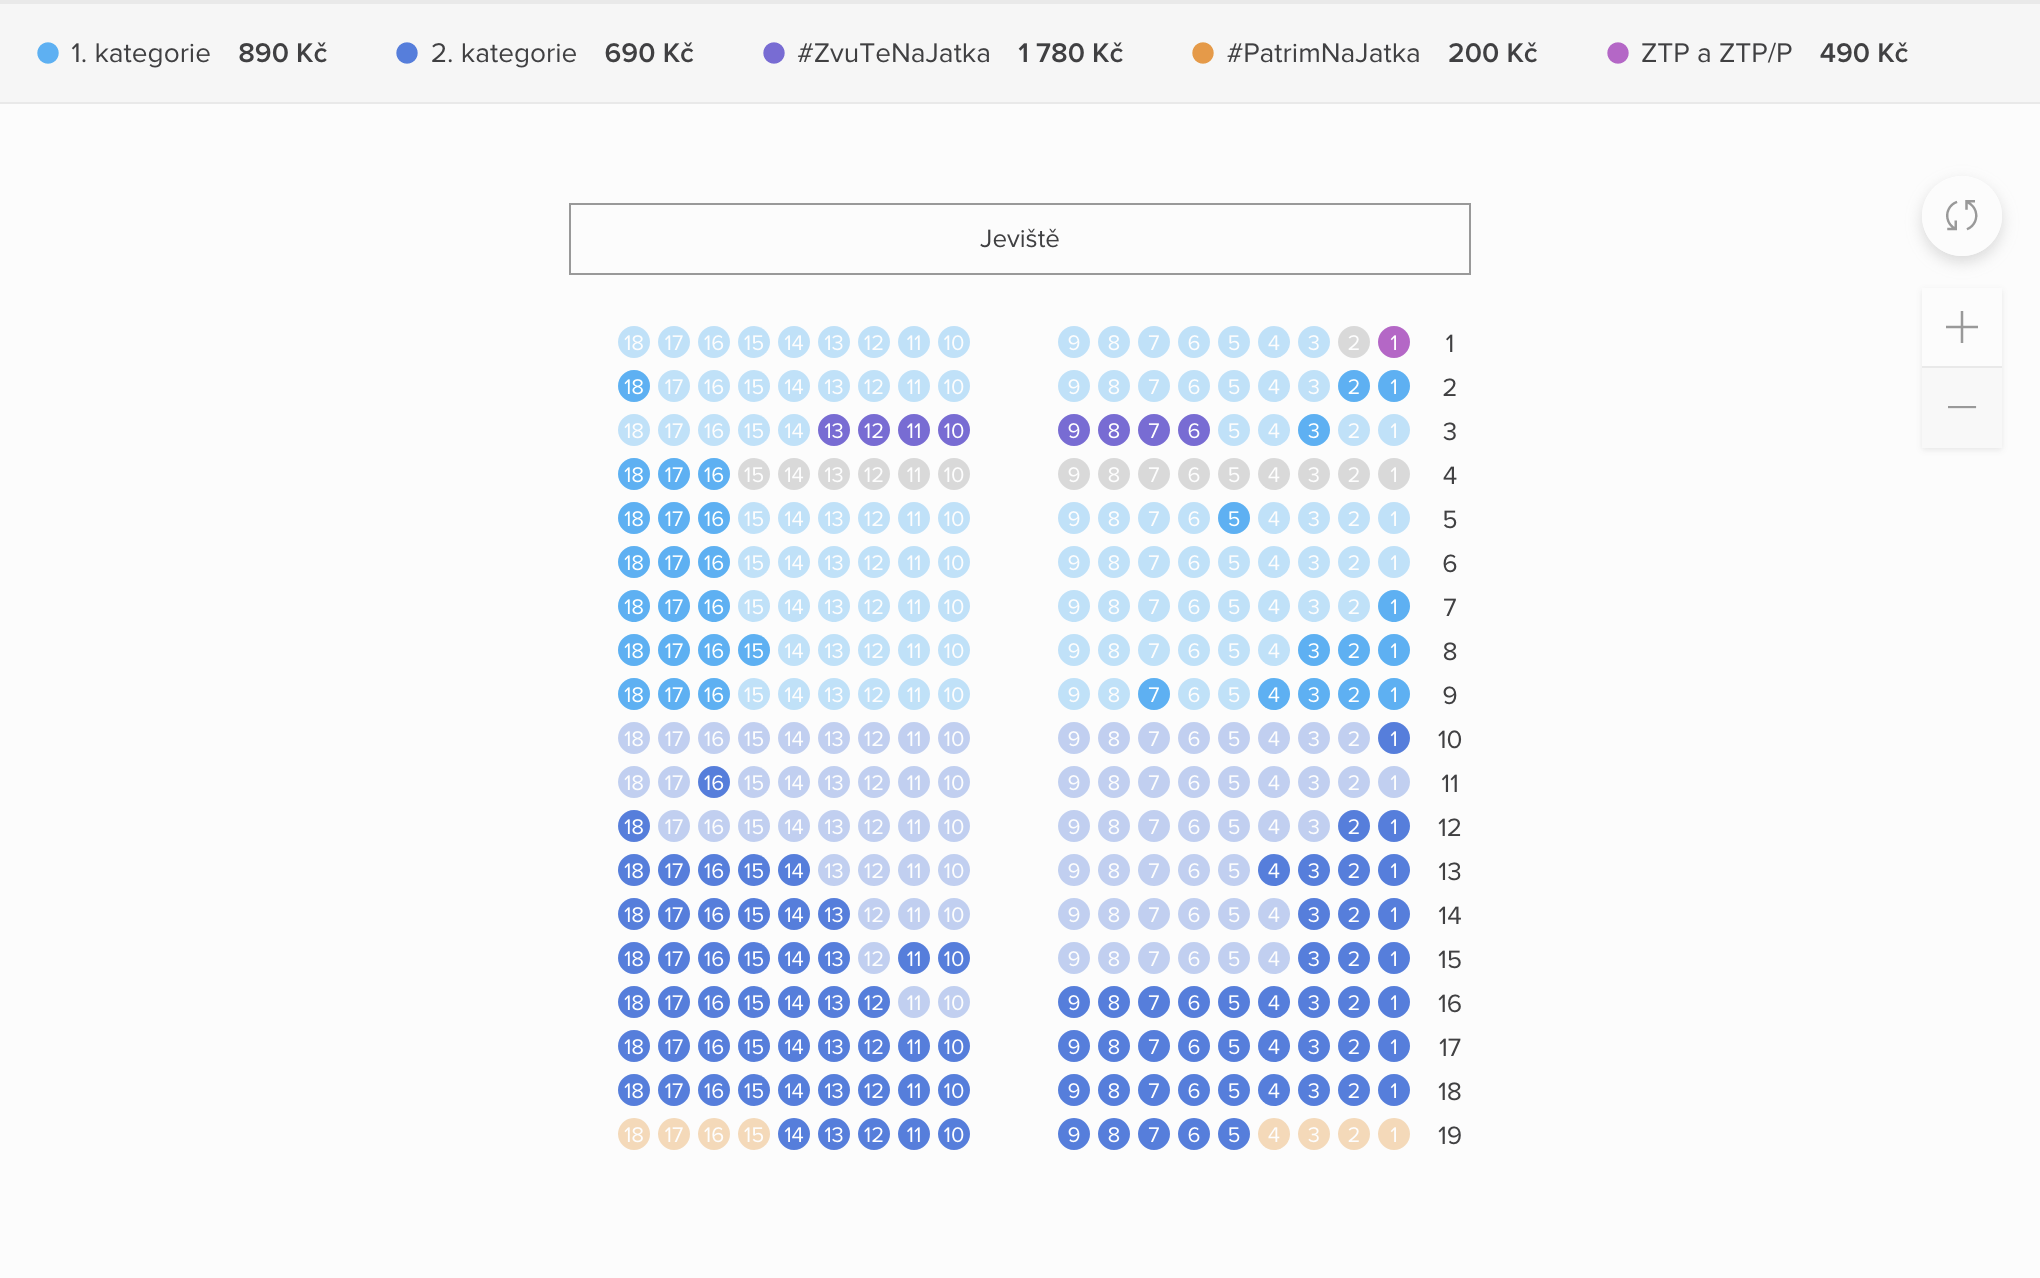
\includegraphics[width=\linewidth]{\FIGDIR/goout-color-codes}
        \centering
        \caption{Mapa barevně odlišených sedadel GoOut\cite{g__goout_net}}
        \label{fig:goout-color-codes}
    \end{figure}

    Efektivní implementace barevného kódování vyžaduje použití snadno rozlišitelných barev, které vyhovují zákazníkům s různými zrakovými schopnostmi.
    Zvolené barevné schéma by mělo zlepšit přehlednost a zvýšit uživatelský komfort tím, že zjednoduší proces výběru sedadel.
    Pro zachování jednotného a přehledného zobrazení je výhodné předem definovat paletu barev, které budou moci být později použity pro různé prvky na mapě.
    Užitím palety barev lze také jednodušeji udržet jednotnou vizuální identitu mapy a lze také předcházet zobrazením nekontrastních barevných kombinací, například textu na barevném podkladu.
\end{subsection}

%%% Podsekce - Ovládání mapy
%%%%% Wording: ✅
%%%%% Styling: ✅
%%%%% References: ✅
%%%%% Grammar: ✅
%%% --------------------------------------------------------------
\begin{subsection}{Ovládání mapy}
    \label{subsec:identifikace-interaktivni-mapa-ovladani}
    Ovládání zobrazení mapy je důležitou částí implementace, jelikož dodává větší interaktivnost tím, že umožňuje například pohyb kamery mapy po ose \em{x} a \em{y}, rotaci či přiblížení a oddálení.
    Tyto funkce zákazníkovi umožňují podrobněji prozkoumat celou mapu místa a zároveň zobrazit více informací na jednom zobrazení.
    Díky těmto funkcím získá zákazník také lepší přehled o celkovém rozpoložení míst v areálu.
    Takovéto funkce jsou esenciální u zobrazení map větších areálů jako jsou například arény či stadiony.
    Tyto mapy jsou totiž většinou ještě rozděleny do sektorů, které seskupují místa k sezení či stání.
    Použitím funkce přiblížení a oddálení lze také zobrazit různé úrovně detailu prvků na mapě v závislosti právě na hodnotě přiblížení.

    Tento přístup například využívá síť Ticketmaster, který je možno vidět na obrázku~\ref{fig:ticketmaster-o2-zoom}, kde je demonstrována mapa sedadel s funkcí přiblížení a posunu a také s rozdělením na sektory.
    Při oddálení mohou uživatelé zobrazit celkové rozložení místa konání rozdělené do sektorů.
    Po přiblížení se zobrazí podrobnější zobrazení jednotlivých míst ve vybraném sektoru, což uživatelům umožňuje podrobně prozkoumat konkrétní oblasti areálu a vybrat požadované místo.

    \begin{figure}[H]
        \centering
        \begin{subfigure}{0.45\textwidth}
            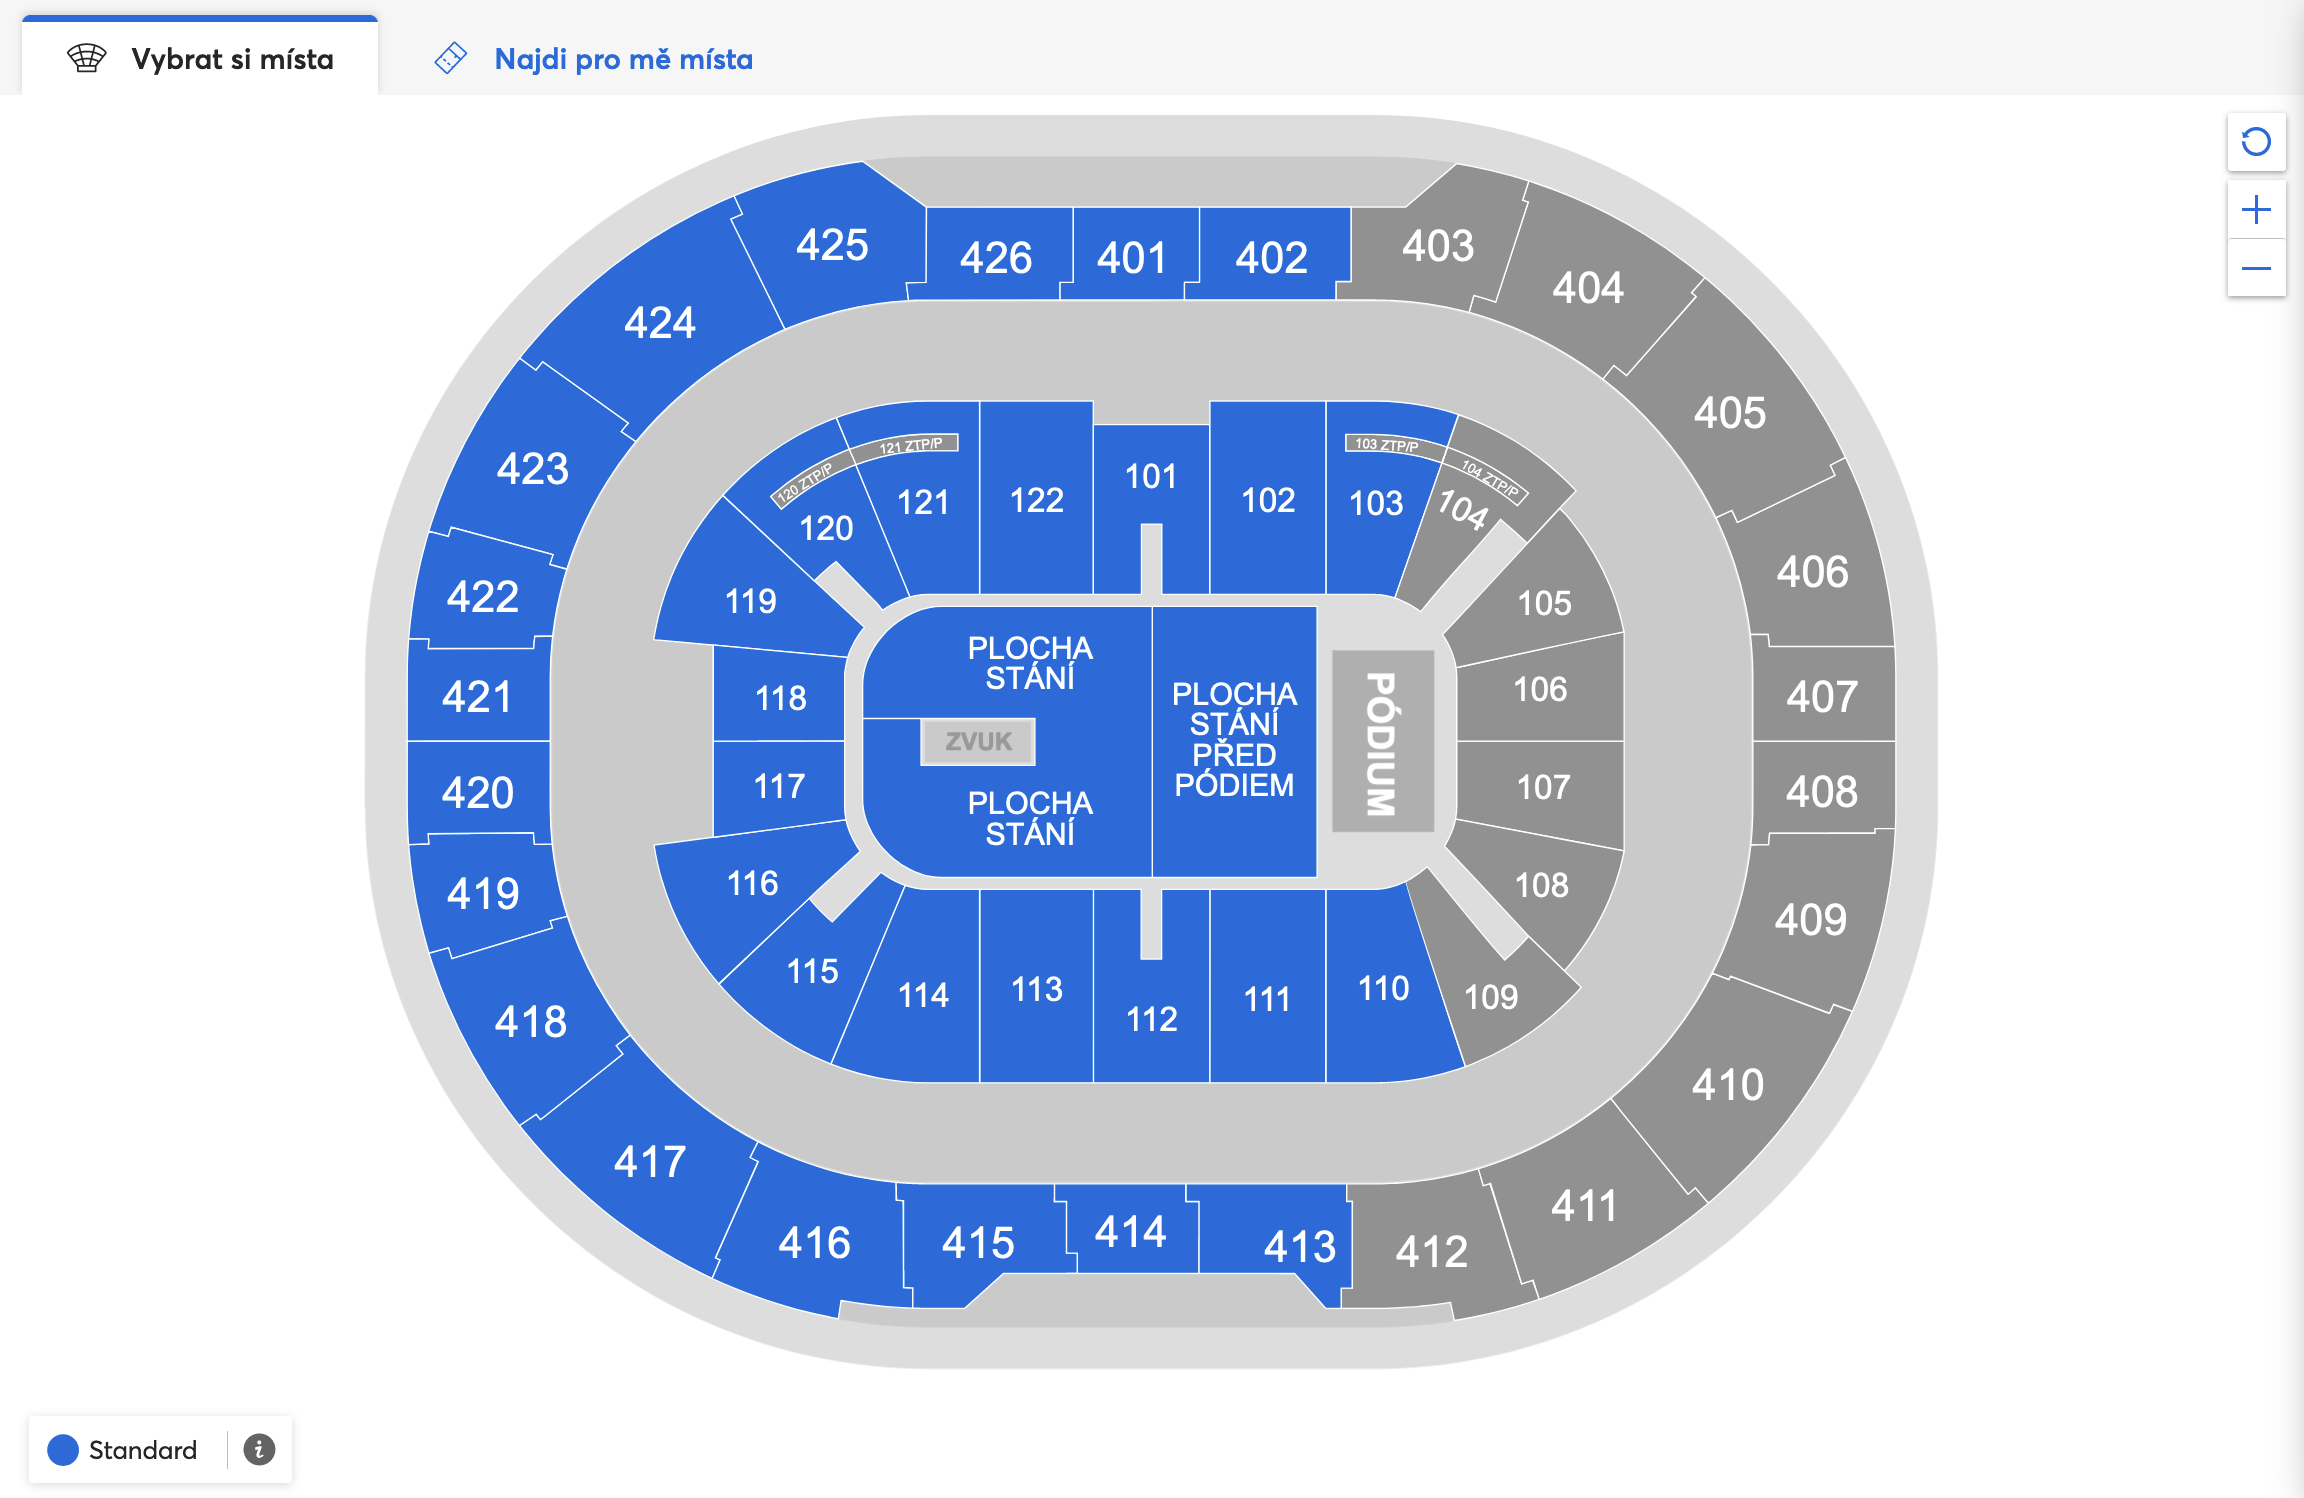
\includegraphics[width=\textwidth]{\FIGDIR/ticketmaster-o2-zoom-out}
            \caption{Oddálený pohled}
            \label{fig:ticketmaster-o2-zoom-in}
        \end{subfigure}
        \hfill
        \begin{subfigure}{0.45\textwidth}
            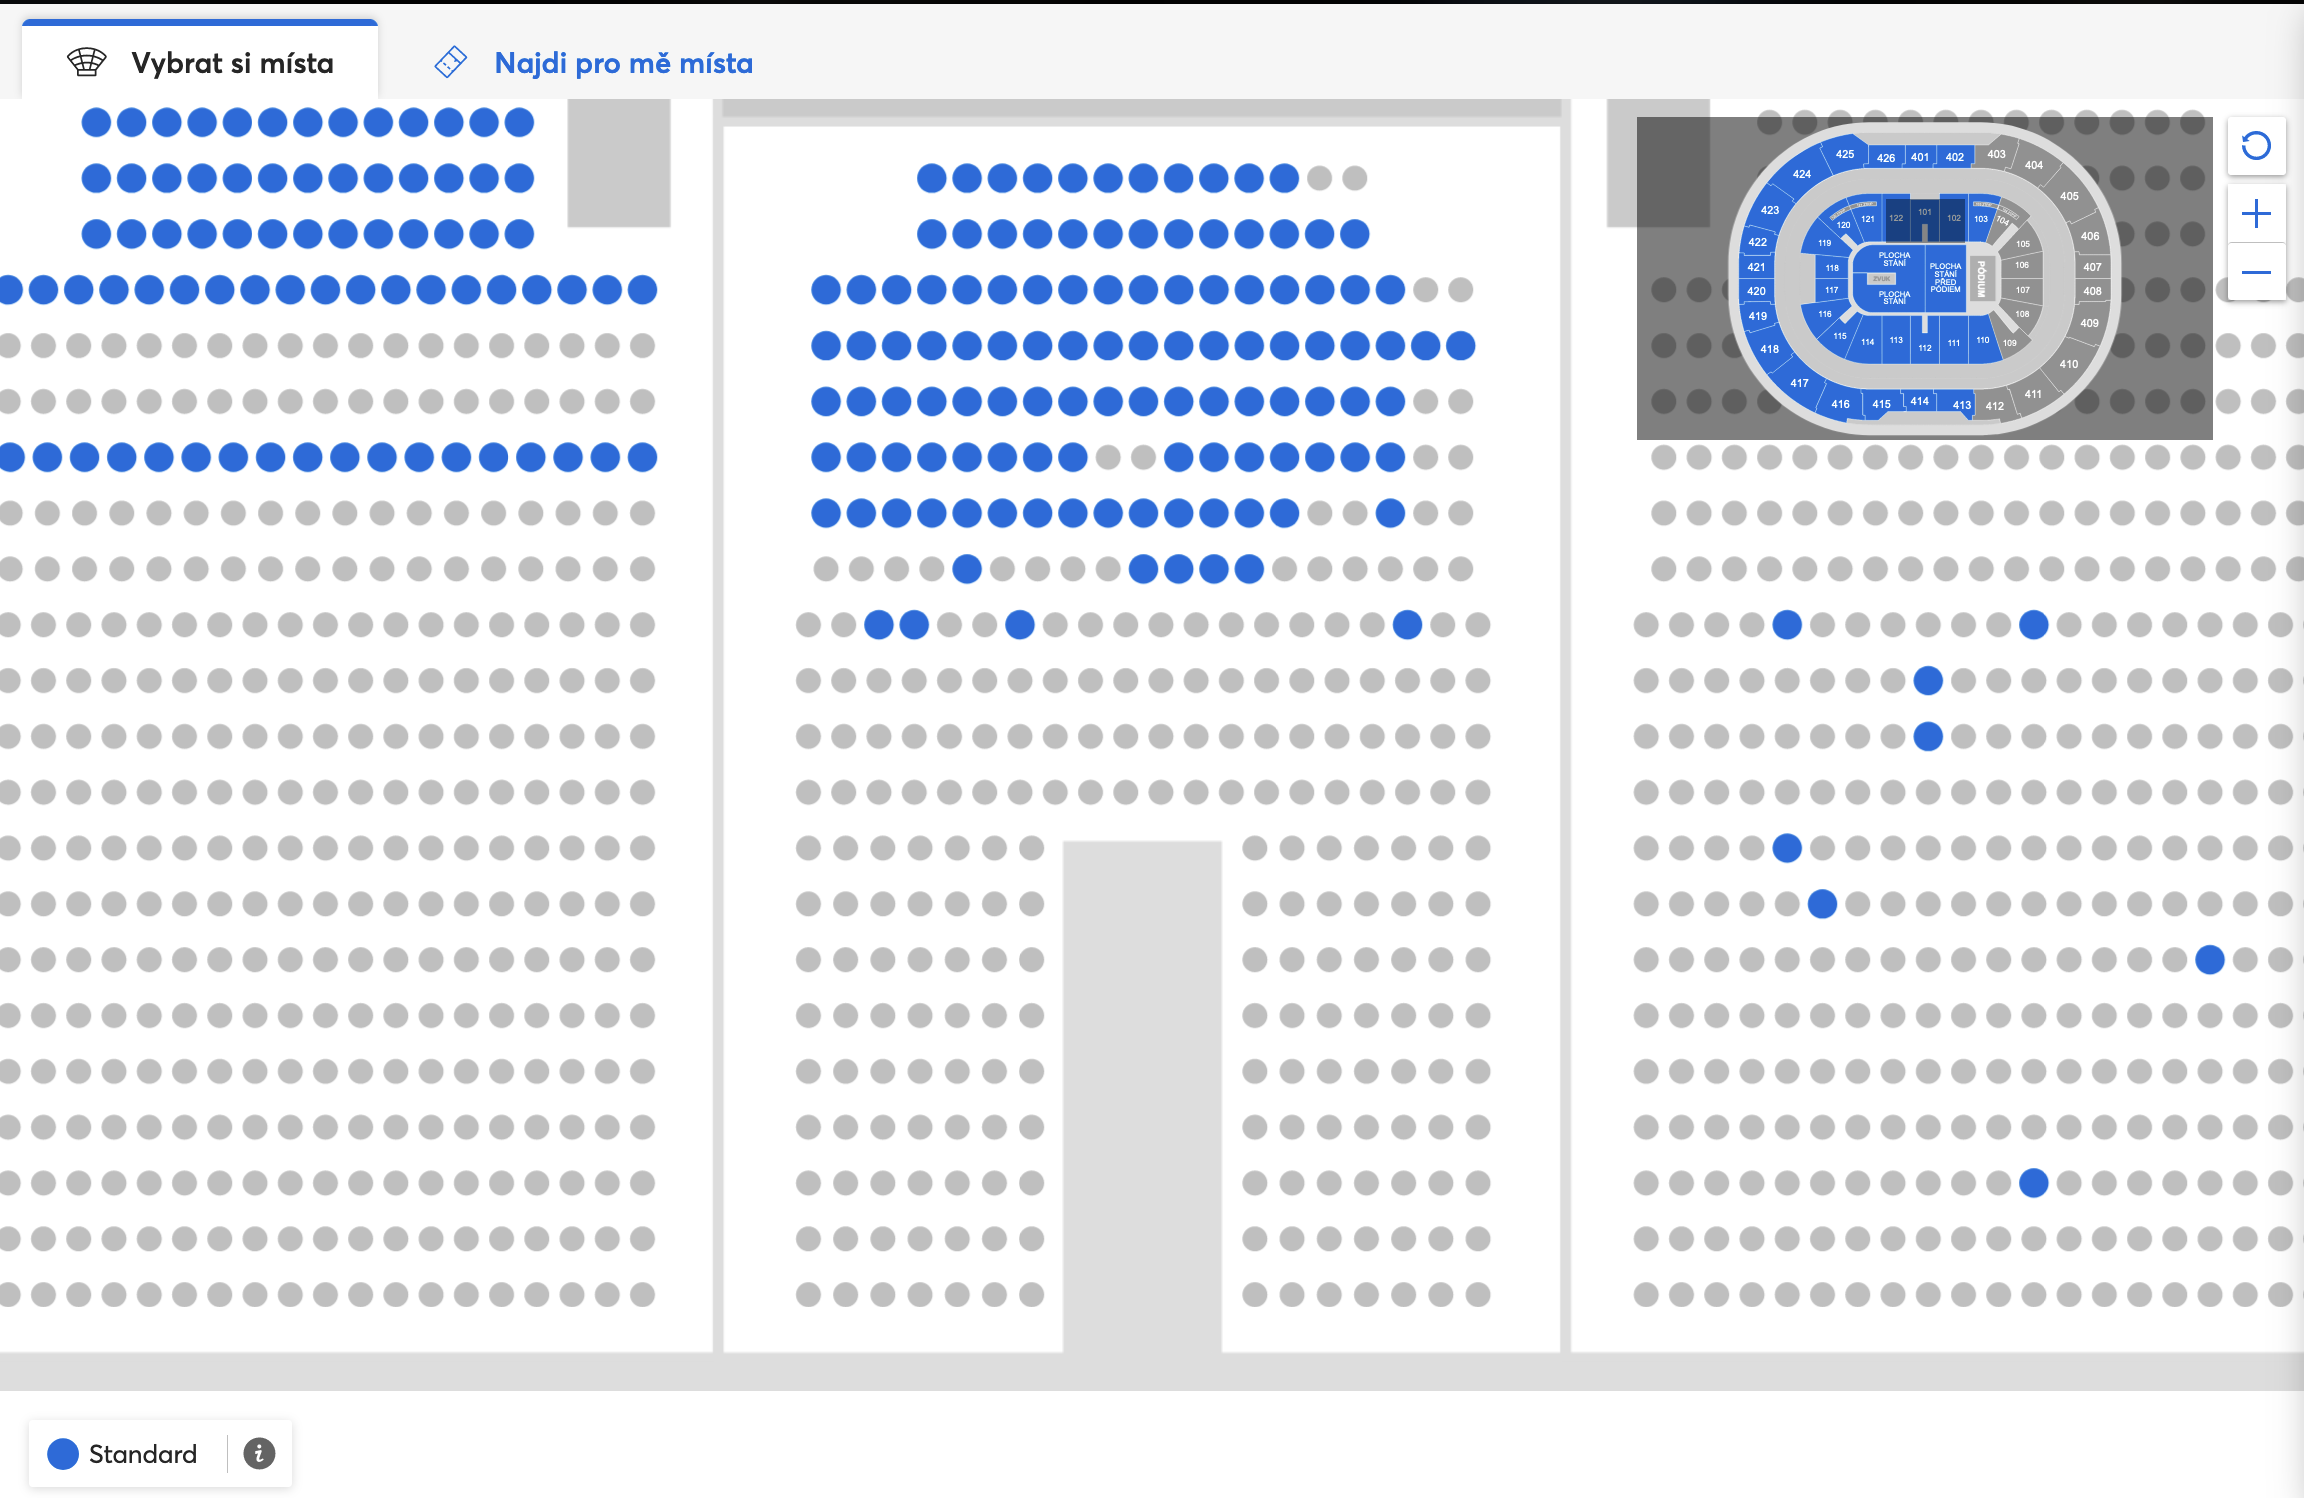
\includegraphics[width=\textwidth]{\FIGDIR/ticketmaster-o2-zoom-in}
            \caption{Přiblížený pohled}
            \label{fig:ticketmaster-o2-zoom-out}
        \end{subfigure}

        \caption{Různé pohledy mapy v síti Ticketmaster.\cite{t__www_ticketmaster_com}}
        \label{fig:ticketmaster-o2-zoom}
    \end{figure}

    Při implementaci těchto funkčností je důležité myslet na přístupnost z pohledu koncových zařízení.
    Například pro nedotyková zařízení tyto funkčnosti zajišťují ukazovací zařízení jako počítačové myši.
    Na dotykových zařízeních jsou tyto funkčnosti docíleny pomocí dotykových gest \foreign{pinch} a \foreign{zoom} pro simulaci přiblížení a oddálení, gesta \foreign{rotate} pro rotaci a gesta \foreign{pan} pro pohyb na osách mapy.
    Je tedy třeba zajistit podporu pro dotyková i nedotyková zařízení.
    Často se k mapám zobrazuje i lišta s nástroji, které tyto funkčnosti ovládají.
    V těchto lištách je také vhodné umístit tlačítko na vrácení zobrazení mapy do výchozího zobrazení.
\end{subsection}

%%% Podsekce - Stav a informace o sedadlech
%%%%% Wording: ✅
%%%%% Styling: ✅
%%%%% References: ✅
%%%%% Grammar: ✅
%%% --------------------------------------------------------------
\begin{subsection}{Stav a informace o sedadlech}
    \label{subsec:identifikace-interaktivni-mapa-stav-a-informace-o-sedadlech}
    Sedadla a ostatní místa k výběru o sobě nesou informace, které na mapě nemusejí být zřejmá a které zákazníkovi usnadňují výběr místa.
    Tyto informace mohou být pro zákazníka zásadní, jelikož poskytují podrobnosti, jako je dostupnost, cena, přístupnost či další jiné popisy.
    Díky těmto informacím se zákazník může lépe rozhodnout a vybrat si sedadlo, které nejlépe vyhovuje jeho preferencím a požadavkům.

    Obrázek~\ref{fig:ticketmaster-o2-seat-info} zobrazuje mapu sedadel se stavem a informacemi o zvoleném sedadlu.
    Uživatelé si mohou zobrazit dostupnost, cenu a další důležité údaje o jednotlivých místech, což jim usnadňuje výběr preferovaných míst k sezení.

    \begin{figure}[H]
        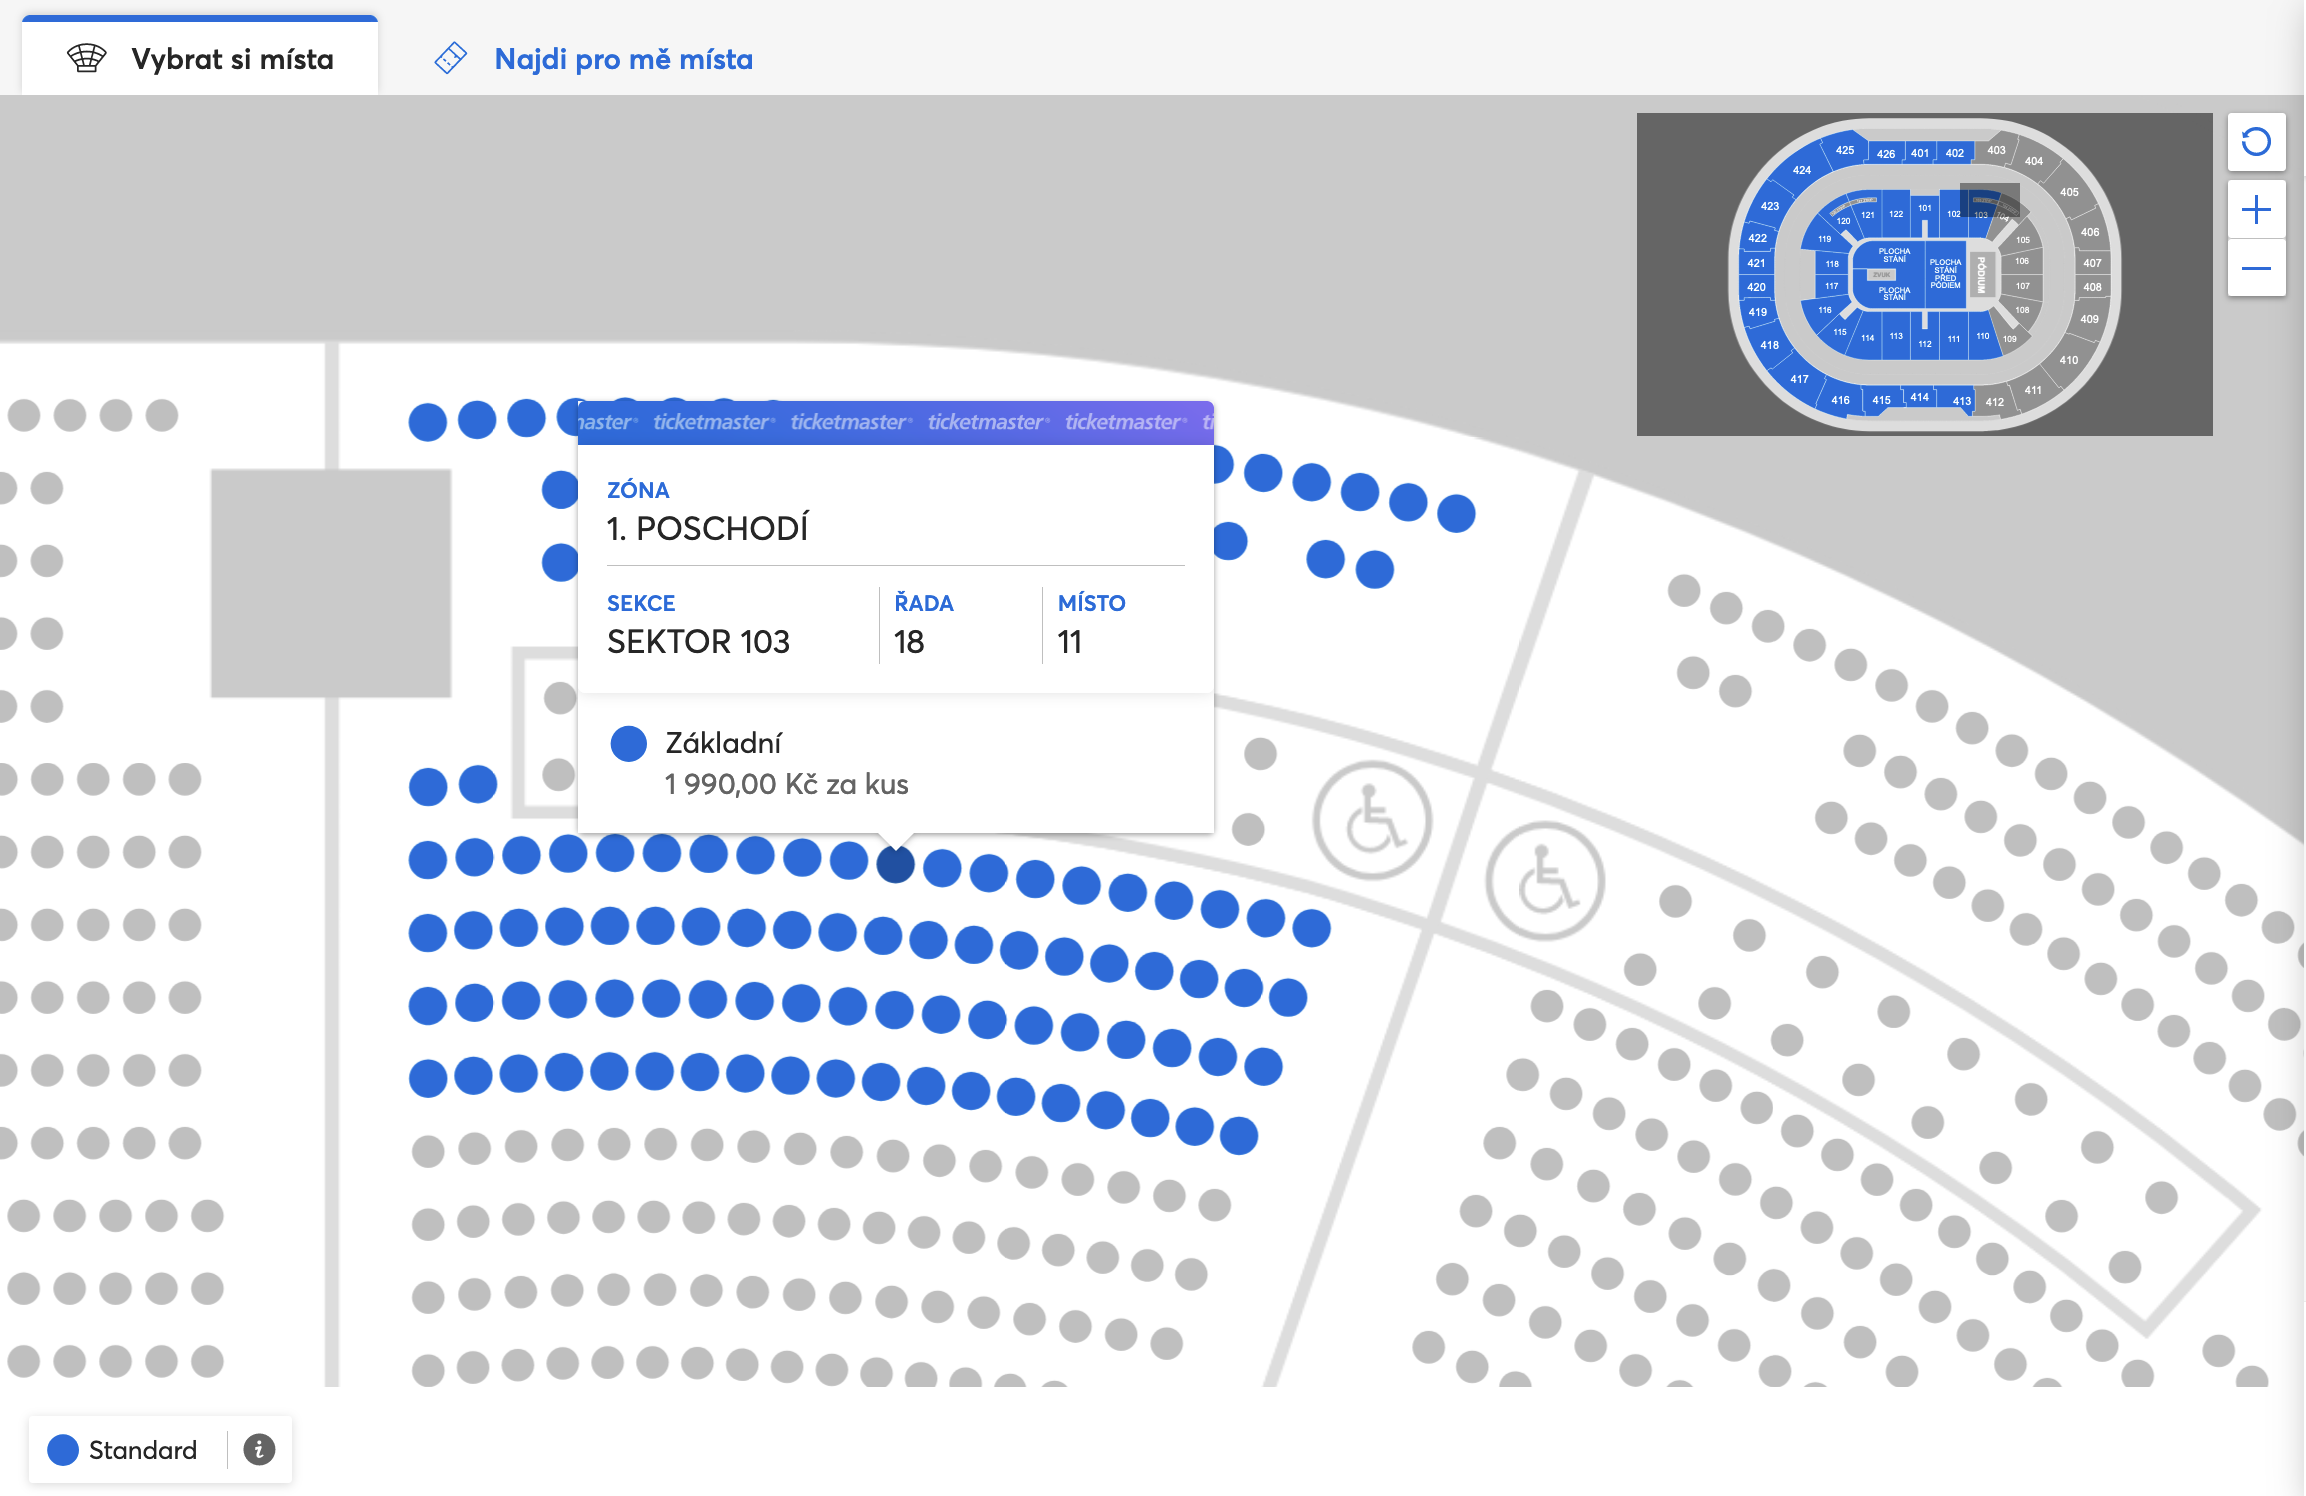
\includegraphics[width=\linewidth]{\FIGDIR/ticketmaster-o2-seat-info}
        \centering
        \caption{Informace o sedadle na mapě v síti Ticketmaster\cite{t__www_ticketmaster_com}}
        \label{fig:ticketmaster-o2-seat-info}
    \end{figure}

    Aby bylo možné efektivně implementovat informace o stavu sedadel, měla by být mapa míst jasná a srozumitelná a všechny důležité údaje by měly být snadno dostupné.
    Jedním z běžných přístupů je použití vyskakovacích oken typu \foreign{popover} s informacemi, které se zobrazí například po najetí myší.
    Tato metoda však nemusí být vhodná pro mobilní a dotyková zařízení, kde takováto podobná gesta nefungují či fungují hodně omezeně.
    Pro řešení tohoto problému lze použít alternativní přístup, a to například zobrazení informací o sedadle ve vyjíždějící spodní či boční liště po označení na sedadla.
    Tím je zajištěno, že stav sedadla a informace o něm jsou přístupné uživatelům na všech zařízeních.

    Toto okno či lišta by měla obsahovat ty nejdůležitější informace o zvoleném místě, jako:
    \begin{enumerate}
        \item \textbf{Řada a místo} – číselné či alfanumerické označení řady a místa sedačky.
        \item \textbf{Sektor} – pokud je mapa rozdělena do sektorů, tak sektor, ve kterém se sedačka nachází.
        \item \textbf{Cenu} – cenu vstupenky odpovídající dané sedačce.
        \item \textbf{Barevné označení} – barevné označení sedačky, například dle její cenové kategorie.
        \item \textbf{Stav sedačky} – stav, ve kterém se sedačka vůči zákazníkovi nachází (obsazená, zvolená, nedostupná, \ldots).
        \item \textbf{Další atributy} – další informativní atributy, jako například informace o zhoršených podmínkách viditelnosti nebo vyhrazení místa pro osoby s postižením.
    \end{enumerate}
\end{subsection}

%%% Podsekce - Data a jejich dostupnost
%%%%% Wording: ✅
%%%%% Styling: ✅
%%%%% References: ✅
%%%%% Grammar: ✅
%%% --------------------------------------------------------------
\begin{subsection}{Data a jejich dostupnost}
    \label{subsec:identifikace-interaktivni-mapa-data-a-dostupnost}
    Pro zobrazení a fungování aplikace je nezbytné mapu a celý její stav zkonstruovat pomocí reálných a aktualizovaných dat dostupných z backendového systému pomocí aplikačního rozhraní, známého jako \ac{api}.
    Tato data obsahují informace o vstupenkách a sedačkách jako například dostupnost, cena, umístění a další ostatní relevantní informace.
    Struktura těchto dat by měla být jasně definovaná a dostupná ve formátu vyhovujícímu užití aplikace.

    Areály s velkým množství sedaček mohou být problematické, a to převážně z pohledu objemu přenášených dat mezi klientem a \ac{api}.
    Je důležité myslet na implementaci inteligentního datového přenosu, který zajistí komunikaci a přenos pouze nezbytných dat.
    Díky menšímu objemu přenášených dat se pak zdá aplikace rychlejší a responsivnější.

    Dalším aspektem práce s daty v takovéto aplikaci je aktualizace dat o dostupnosti.
    Tato funkčnost zajišťuje zákazníkovi zobrazení aktuálních informací o sedačkách či vstupenkách a snižuje tak například riziko konfliktu výběru již obsazené sedačky.
    Průběžné aktualizace dat lze docílit technologiemi jako například \foreign{WebSockets} nebo částečnými aktualizacemi dotazovanými skrze \ac{api}.
\end{subsection}
